\documentclass[12pt, a4paper]{article}

% ─── Packages ──────────────────────────────────────────────────────────────────
\usepackage[T1]{fontenc}
\usepackage[utf8]{inputenc}
\usepackage{lmodern}
\usepackage[margin=2.5cm]{geometry}
\usepackage{graphicx}
\usepackage{booktabs}
\usepackage{array}
\usepackage{tabularx}
\usepackage{xcolor}
\usepackage{amsmath}
\usepackage{amssymb}
\usepackage{hyperref}
\usepackage{caption}
\usepackage{subcaption}
\usepackage{float}
\usepackage{parskip}
\usepackage{titlesec}
\usepackage{fancyhdr}
\usepackage{listings}
\usepackage{microtype}

% ─── Colours ───────────────────────────────────────────────────────────────────
\definecolor{accent}{RGB}{0,86,179}
\definecolor{lightgray}{RGB}{245,245,245}
\definecolor{codegray}{RGB}{100,100,100}

% ─── Hyperref ──────────────────────────────────────────────────────────────────
\hypersetup{
    colorlinks=true,
    linkcolor=accent,
    urlcolor=accent,
    citecolor=accent,
    pdftitle={Diabetes Dataset: EDA and Prediction},
    pdfauthor={Tommi Bimbato}
}

% ─── Header / Footer ───────────────────────────────────────────────────────────
\pagestyle{fancy}
\fancyhf{}
\fancyhead[L]{\small Diabetes Dataset: EDA \& Prediction}
\fancyhead[R]{\small Model Benchmark Report}
\fancyfoot[C]{\thepage}
\renewcommand{\headrulewidth}{0.4pt}

% ─── Section styling ───────────────────────────────────────────────────────────
\titleformat{\section}{\large\bfseries\color{accent}}{}{0em}{\thesection\quad}[\titlerule]
\titleformat{\subsection}{\normalsize\bfseries}{}{0em}{\thesubsection\quad}

% ─── Graphics path ─────────────────────────────────────────────────────────────
\graphicspath{{../figures/eda/}{../figures/pred/}}

% ─── Listings ──────────────────────────────────────────────────────────────────
\lstset{
    backgroundcolor=\color{lightgray},
    basicstyle=\ttfamily\footnotesize,
    breaklines=true,
    frame=single,
    rulecolor=\color{codegray},
    numbers=none
}

% ══════════════════════════════════════════════════════════════════════════════
\begin{document}

% ─── Title page ──────────────────────────────────────────────────────────────
\begin{titlepage}
    \centering
    \vspace*{2cm}
    {\Huge\bfseries\color{accent} Diabetes Dataset\\[0.4em]
     Exploratory Data Analysis\\[0.4em]
     \& Predictive Modelling\par}
    \vspace{1.5cm}
      {\large\itshape Comparative Benchmark of 4 Classification Models\par}
    \vspace{0.5cm}

    \vspace{2cm}
    \rule{0.5\textwidth}{0.4pt}\\[0.5cm]
    {\Large Tommi Bimbato\par}
    \vspace{0.5cm}
    {\normalsize\today\par}
    \vfill
    \small\textit{This project is purely educational. Results must not be used
    for medical diagnosis or treatment.}
\end{titlepage}

% ─── Table of contents ───────────────────────────────────────────────────────
\tableofcontents
\newpage

% ══════════════════════════════════════════════════════════════════════════════
\section{Introduction}

This report documents a complete data science pipeline applied to a real-world
diabetes dataset. The objective is to benchmark four classification algorithms
(Logistic Regression, Decision Tree, KNN, Random Forest) under both imbalanced
and balanced training conditions, and to package the full workflow in an
interactive Streamlit interface.

\subsection{Executive Summary}

Key outcomes of this benchmark are:
\begin{itemize}
    \item \textbf{Top performance above 98\%}: Decision Tree and Random Forest
          both reached \textbf{99.5\% accuracy} on the held-out test set.
    \item \textbf{Clinical-feature signal is strong}: HbA1c, BMI, and AGE
          emerge consistently as the most informative predictors.
    \item \textbf{Balancing improves minority-class recall}: for example,
          Logistic Regression Recall (0) improves from 0.750 to 0.950 after
          random undersampling.
\end{itemize}

The work is organised into four main phases:
\begin{enumerate}
    \item \textbf{Data cleaning and preprocessing} --- handling null values,
          encoding categorical features, and detecting physiologically
          implausible outliers.
    \item \textbf{Exploratory Data Analysis (EDA)} --- understanding feature
          distributions, class balance, and inter-feature correlations.
    \item \textbf{Predictive modelling} --- training and comparing four
          classification algorithms on both the original (imbalanced) and an
          undersampled (balanced) training set.
    \item \textbf{Interactive web application} --- a Streamlit app that exposes
          the full pipeline and allows real-time predictions from user-supplied
          patient data.
\end{enumerate}

\subsection{Dataset}

The raw dataset \texttt{diabetes\_unclean.csv} was sourced from
\href{https://www.kaggle.com/datasets/kabirolawalemohammed/diabetes-unclean}{Kaggle}
and contains 1\,009 patient records with 14 columns.
Table~\ref{tab:features} describes each feature.

\begin{table}[H]
\centering
\caption{Dataset features and descriptions.}
\label{tab:features}
\renewcommand{\arraystretch}{1.3}
\begin{tabularx}{\textwidth}{lX}
\toprule
\textbf{Feature} & \textbf{Description} \\
\midrule
Gender  & Patient gender (M/F) \\
AGE     & Age in years \\
Urea    & Blood urea level (mmol/L) --- kidney function indicator \\
Cr      & Creatinine level (µmol/L) --- kidney function indicator \\
HbA1c   & Glycated haemoglobin (\%) --- average blood glucose over 3 months \\
Chol    & Total cholesterol (mmol/L) \\
TG      & Triglycerides (mmol/L) \\
HDL     & High-density lipoprotein (mmol/L) --- ``good cholesterol'' \\
LDL     & Low-density lipoprotein (mmol/L) --- ``bad cholesterol'' \\
VLDL    & Very low-density lipoprotein (mmol/L) \\
BMI     & Body Mass Index (kg/m\textsuperscript{2}) \\
CLASS   & Target: 1 = diabetic, 0 = non-diabetic \\
\bottomrule
\end{tabularx}
\end{table}

% ══════════════════════════════════════════════════════════════════════════════
\section{Data Cleaning and Preprocessing}

\subsection{Null Values}

The raw dataset contained a small number of missing values (less than 2\% of
rows). Given this negligible proportion, affected rows were simply dropped
rather than imputed, preserving data integrity without significant information
loss.

\subsection{Categorical Encoding}

Two columns required encoding before numerical analysis could proceed:

\begin{itemize}
    \item \textbf{Gender} --- inconsistent casing (\texttt{m}, \texttt{M},
          \texttt{f}, \texttt{F}) was normalised and mapped to
          $0 = \text{Male}$, $1 = \text{Female}$.
    \item \textbf{CLASS} --- contained mixed values (\texttt{Y}, \texttt{N},
          \texttt{P}, padded spaces). After stripping and uppercasing,
          \texttt{P} was remapped to \texttt{Y}, then encoded as
          $1 = \text{Diabetic}$, $0 = \text{Non-diabetic}$.
\end{itemize}

\subsection{Removal of Irrelevant Columns}

Columns \texttt{ID} and \texttt{No\_Pation} are administrative identifiers
with no predictive value and were therefore removed.

\subsection{Outlier Detection}

A standard-deviation criterion was adopted to flag features with potentially
anomalous variance:
\[
    \text{Flag if:}\quad \sigma > \frac{\mu}{2}
\]
This identified five features with abnormally high dispersion: \textbf{Urea},
\textbf{Cr}, \textbf{TG}, \textbf{HDL}, and \textbf{VLDL}.

Physiologically motivated thresholds (Table~\ref{tab:outlier}) were then applied
to replace values outside biologically plausible ranges with \texttt{NaN},
which were subsequently dropped.

\begin{table}[H]
\centering
\caption{Physiological thresholds used for outlier removal.
         \textit{Disclaimer: values obtained from online sources for
         illustrative purposes only; not medically validated.}}
\label{tab:outlier}
\renewcommand{\arraystretch}{1.3}
\begin{tabular}{llll}
\toprule
\textbf{Feature} & \textbf{Lower limit} & \textbf{Upper limit} & \textbf{Unit} \\
\midrule
Urea  & 1    & 25  & mmol/L \\
Cr    & 10   & 400 & µmol/L \\
TG    & 0.1  & 10  & mmol/L \\
HDL   & 0.3  & 5   & mmol/L \\
VLDL  & 0.05 & 40  & mmol/L \\
\bottomrule
\end{tabular}
\end{table}

Figure~\ref{fig:boxplots_suspicious} shows the distribution of flagged features
with threshold lines superimposed.

\begin{figure}[H]
    \centering
    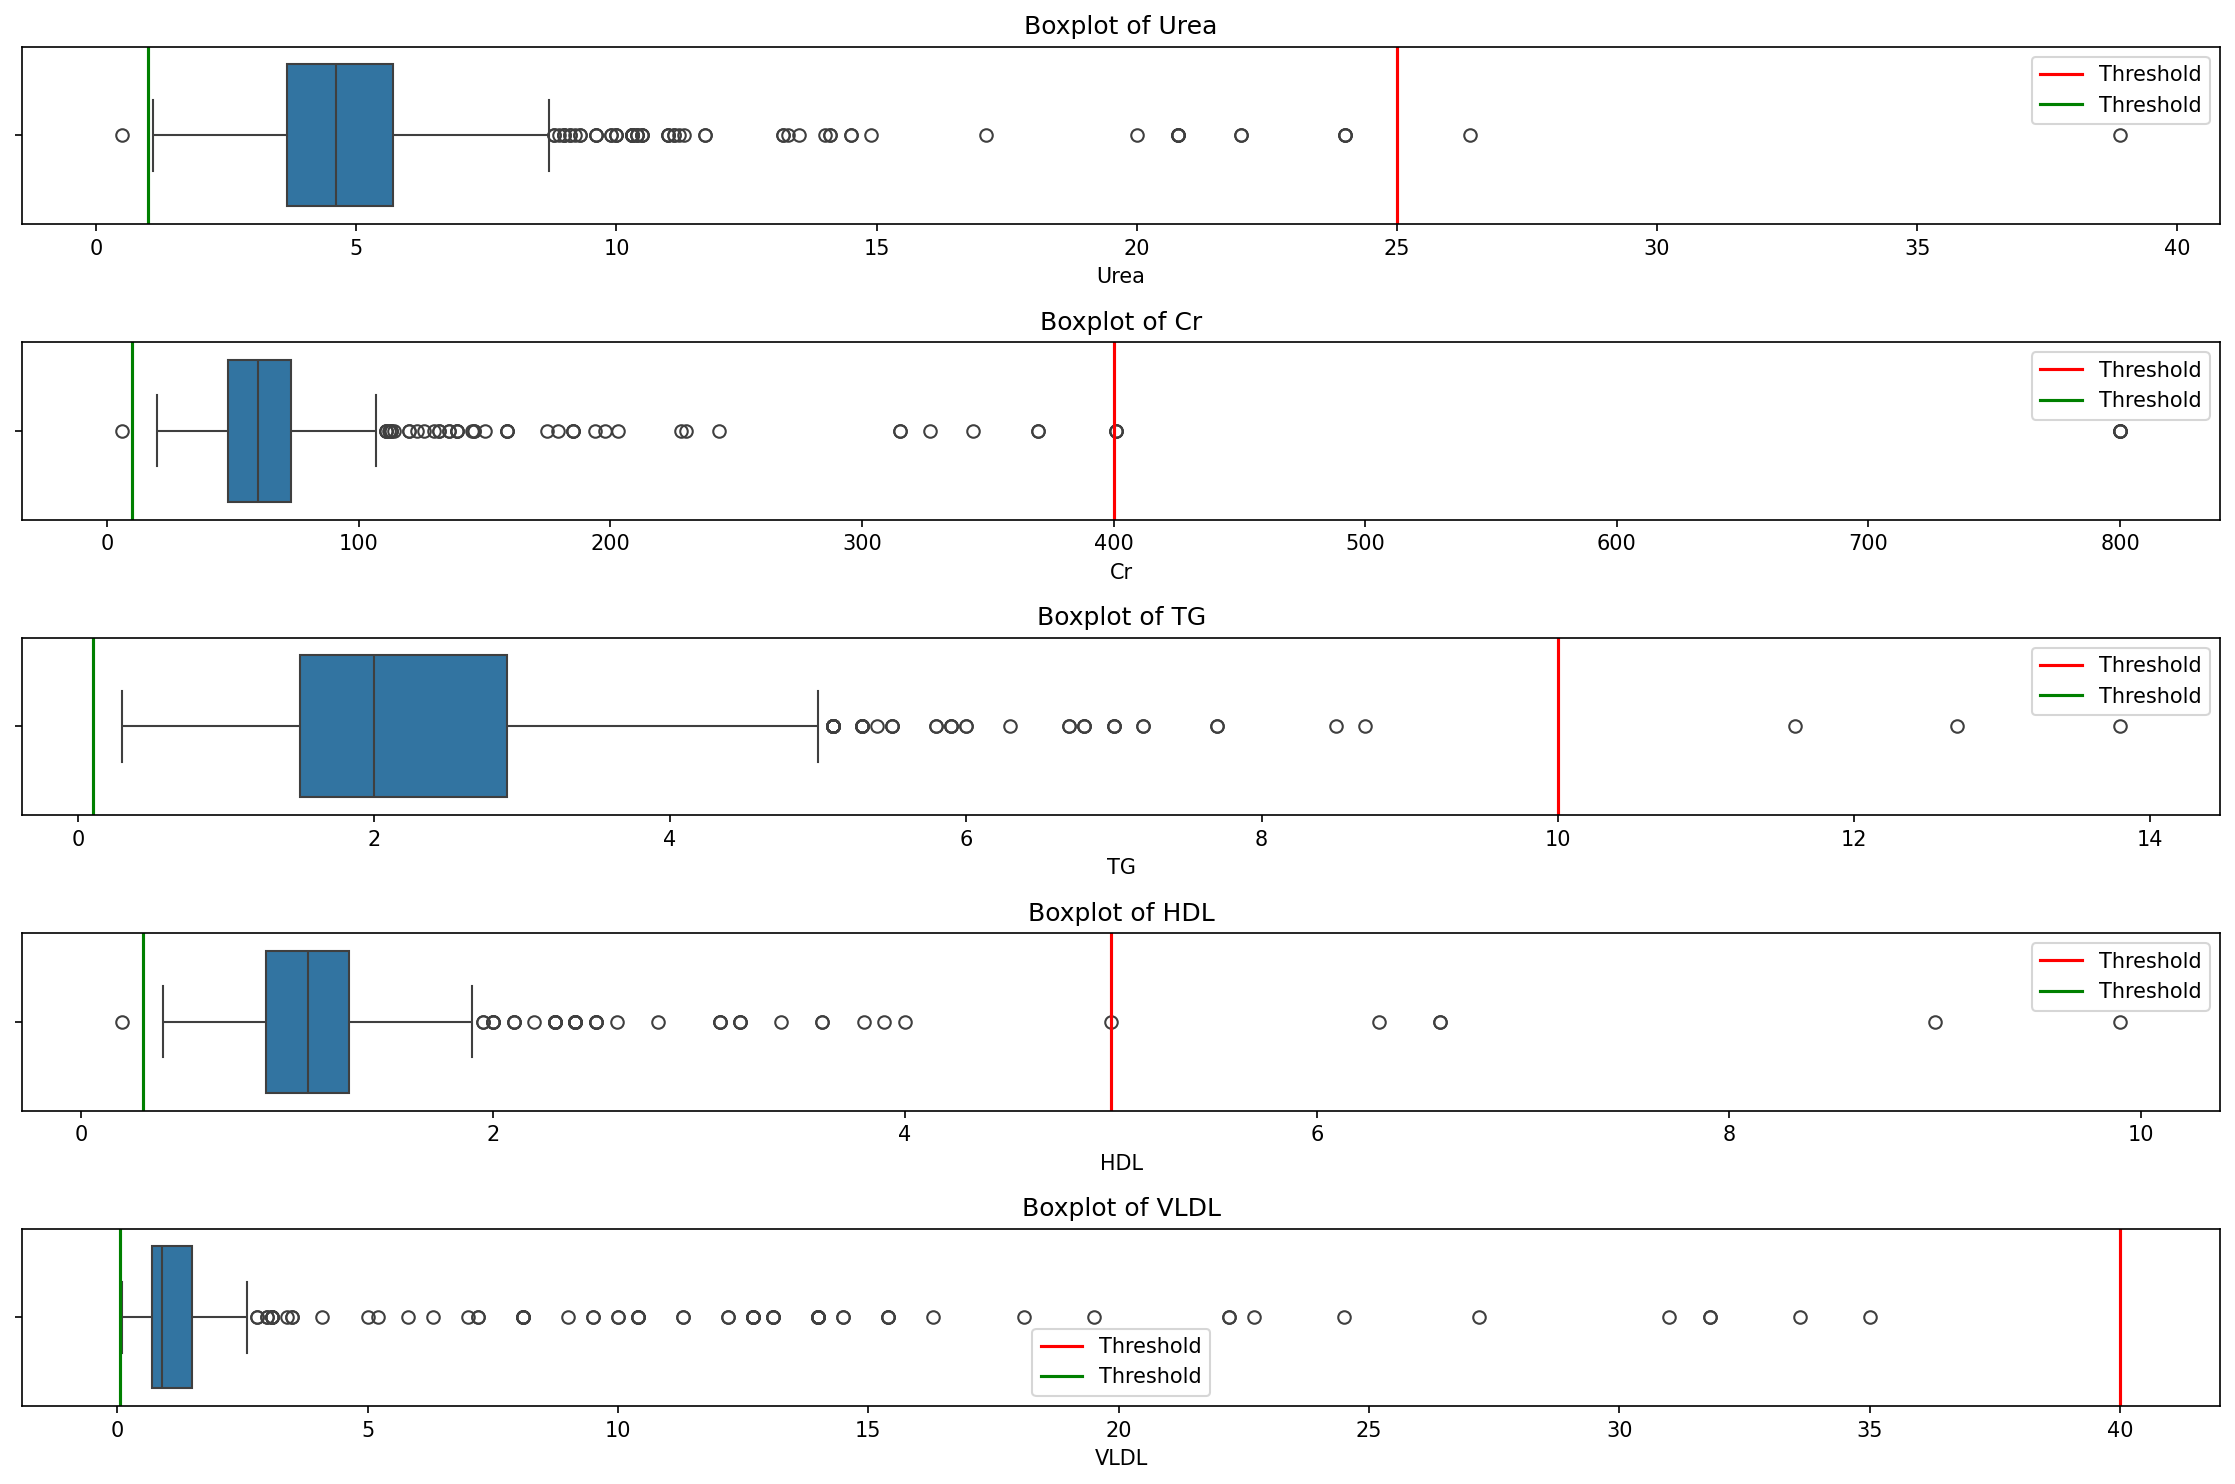
\includegraphics[width=\textwidth]{03_suspicious_features_boxplots.png}
    \caption{Horizontal boxplots for the five high-variance features. Red lines
             mark upper physiological limits; green lines mark lower limits.}
    \label{fig:boxplots_suspicious}
\end{figure}

\subsection{VLDL Unit Inconsistency}

Scatter plots of TG versus VLDL revealed two distinct clusters
(Figure~\ref{fig:vldl_before}): one group following the expected synthetic
relationship $\text{VLDL} = \text{TG} / 2.2$ (mmol/L), and a second group
with values above 4 that followed a different scaling --- later identified as
measurements recorded in mg/dL rather than mmol/L.

\begin{figure}[H]
    \centering
    \begin{subfigure}[b]{0.48\textwidth}
        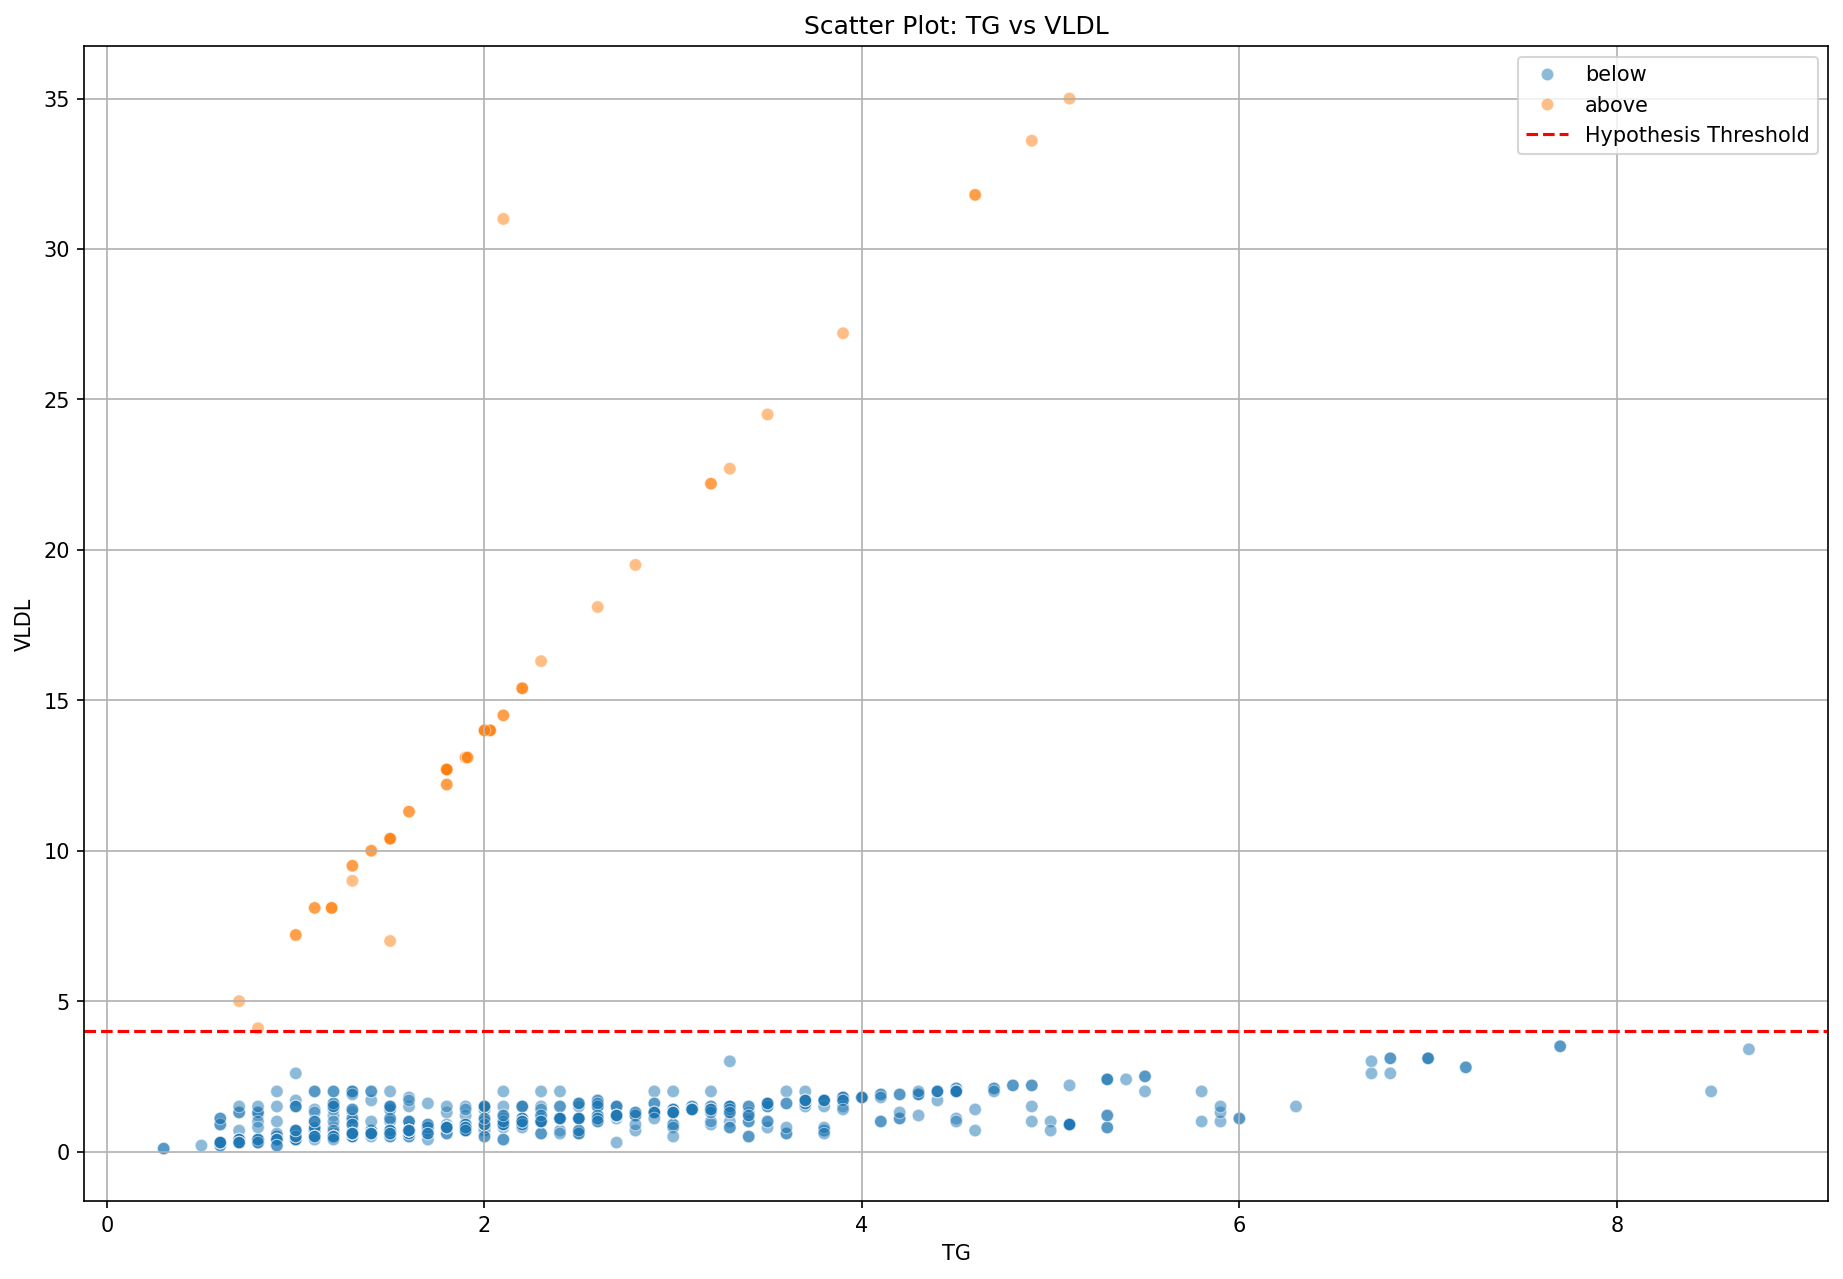
\includegraphics[width=\textwidth]{04_tg_vldl_scatter.png}
        \caption{Before correction: two distinct groups visible.}
        \label{fig:vldl_before}
    \end{subfigure}
    \hfill
    \begin{subfigure}[b]{0.48\textwidth}
        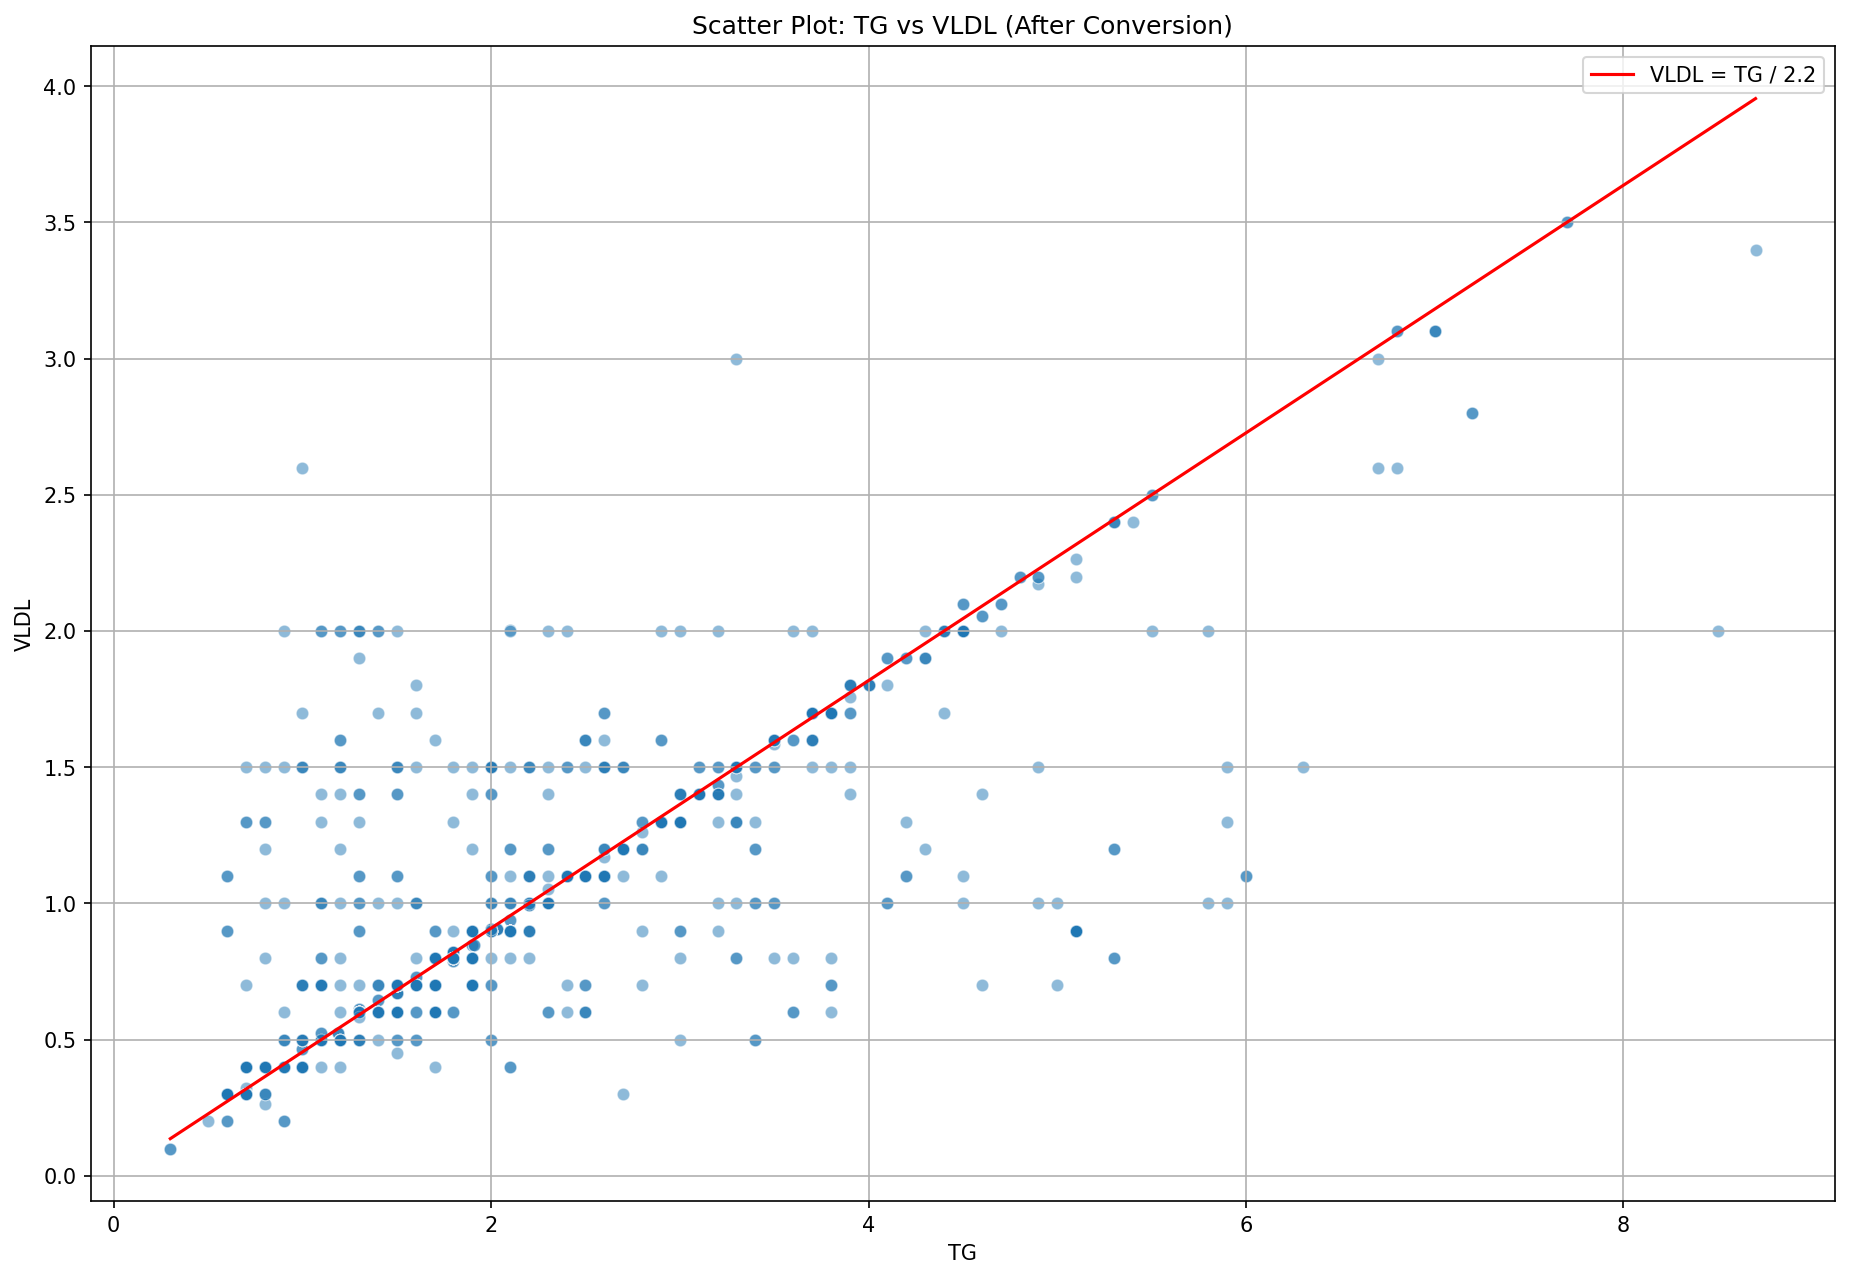
\includegraphics[width=\textwidth]{07_tg_vldl_after_correction.png}
        \caption{After unit correction: all values follow $\text{VLDL} = \text{TG}/2.2$.}
        \label{fig:vldl_after}
    \end{subfigure}
    \caption{TG vs.\ VLDL scatter plots before and after unit correction.}
\end{figure}

The conversion applied to values $\text{VLDL} > 4$ was:
\[
    \text{VLDL}_{\text{mmol/L}}
    = \frac{\text{VLDL}_{\text{mg/dL}} \times 5.5}{38.67 \times 2.2}
\]

After all cleaning steps the dataset comprised \textbf{974 patient records}
ready for analysis.

% ══════════════════════════════════════════════════════════════════════════════
\section{Exploratory Data Analysis}

\subsection{Class Distribution}

The cleaned dataset is highly imbalanced: 89.5\% of patients (872 out of 974)
are diabetic (CLASS = 1), while only 10.5\% (102 patients) are non-diabetic
(CLASS = 0). This imbalance directly motivates the need for dataset balancing
before model training, discussed in Section~\ref{sec:balancing}.

\subsection{Feature Distributions}

Figure~\ref{fig:all_boxplots} presents horizontal boxplots for all numeric
features, offering a concise summary of their spread and the presence of
residual extreme values after outlier removal.

\begin{figure}[H]
    \centering
    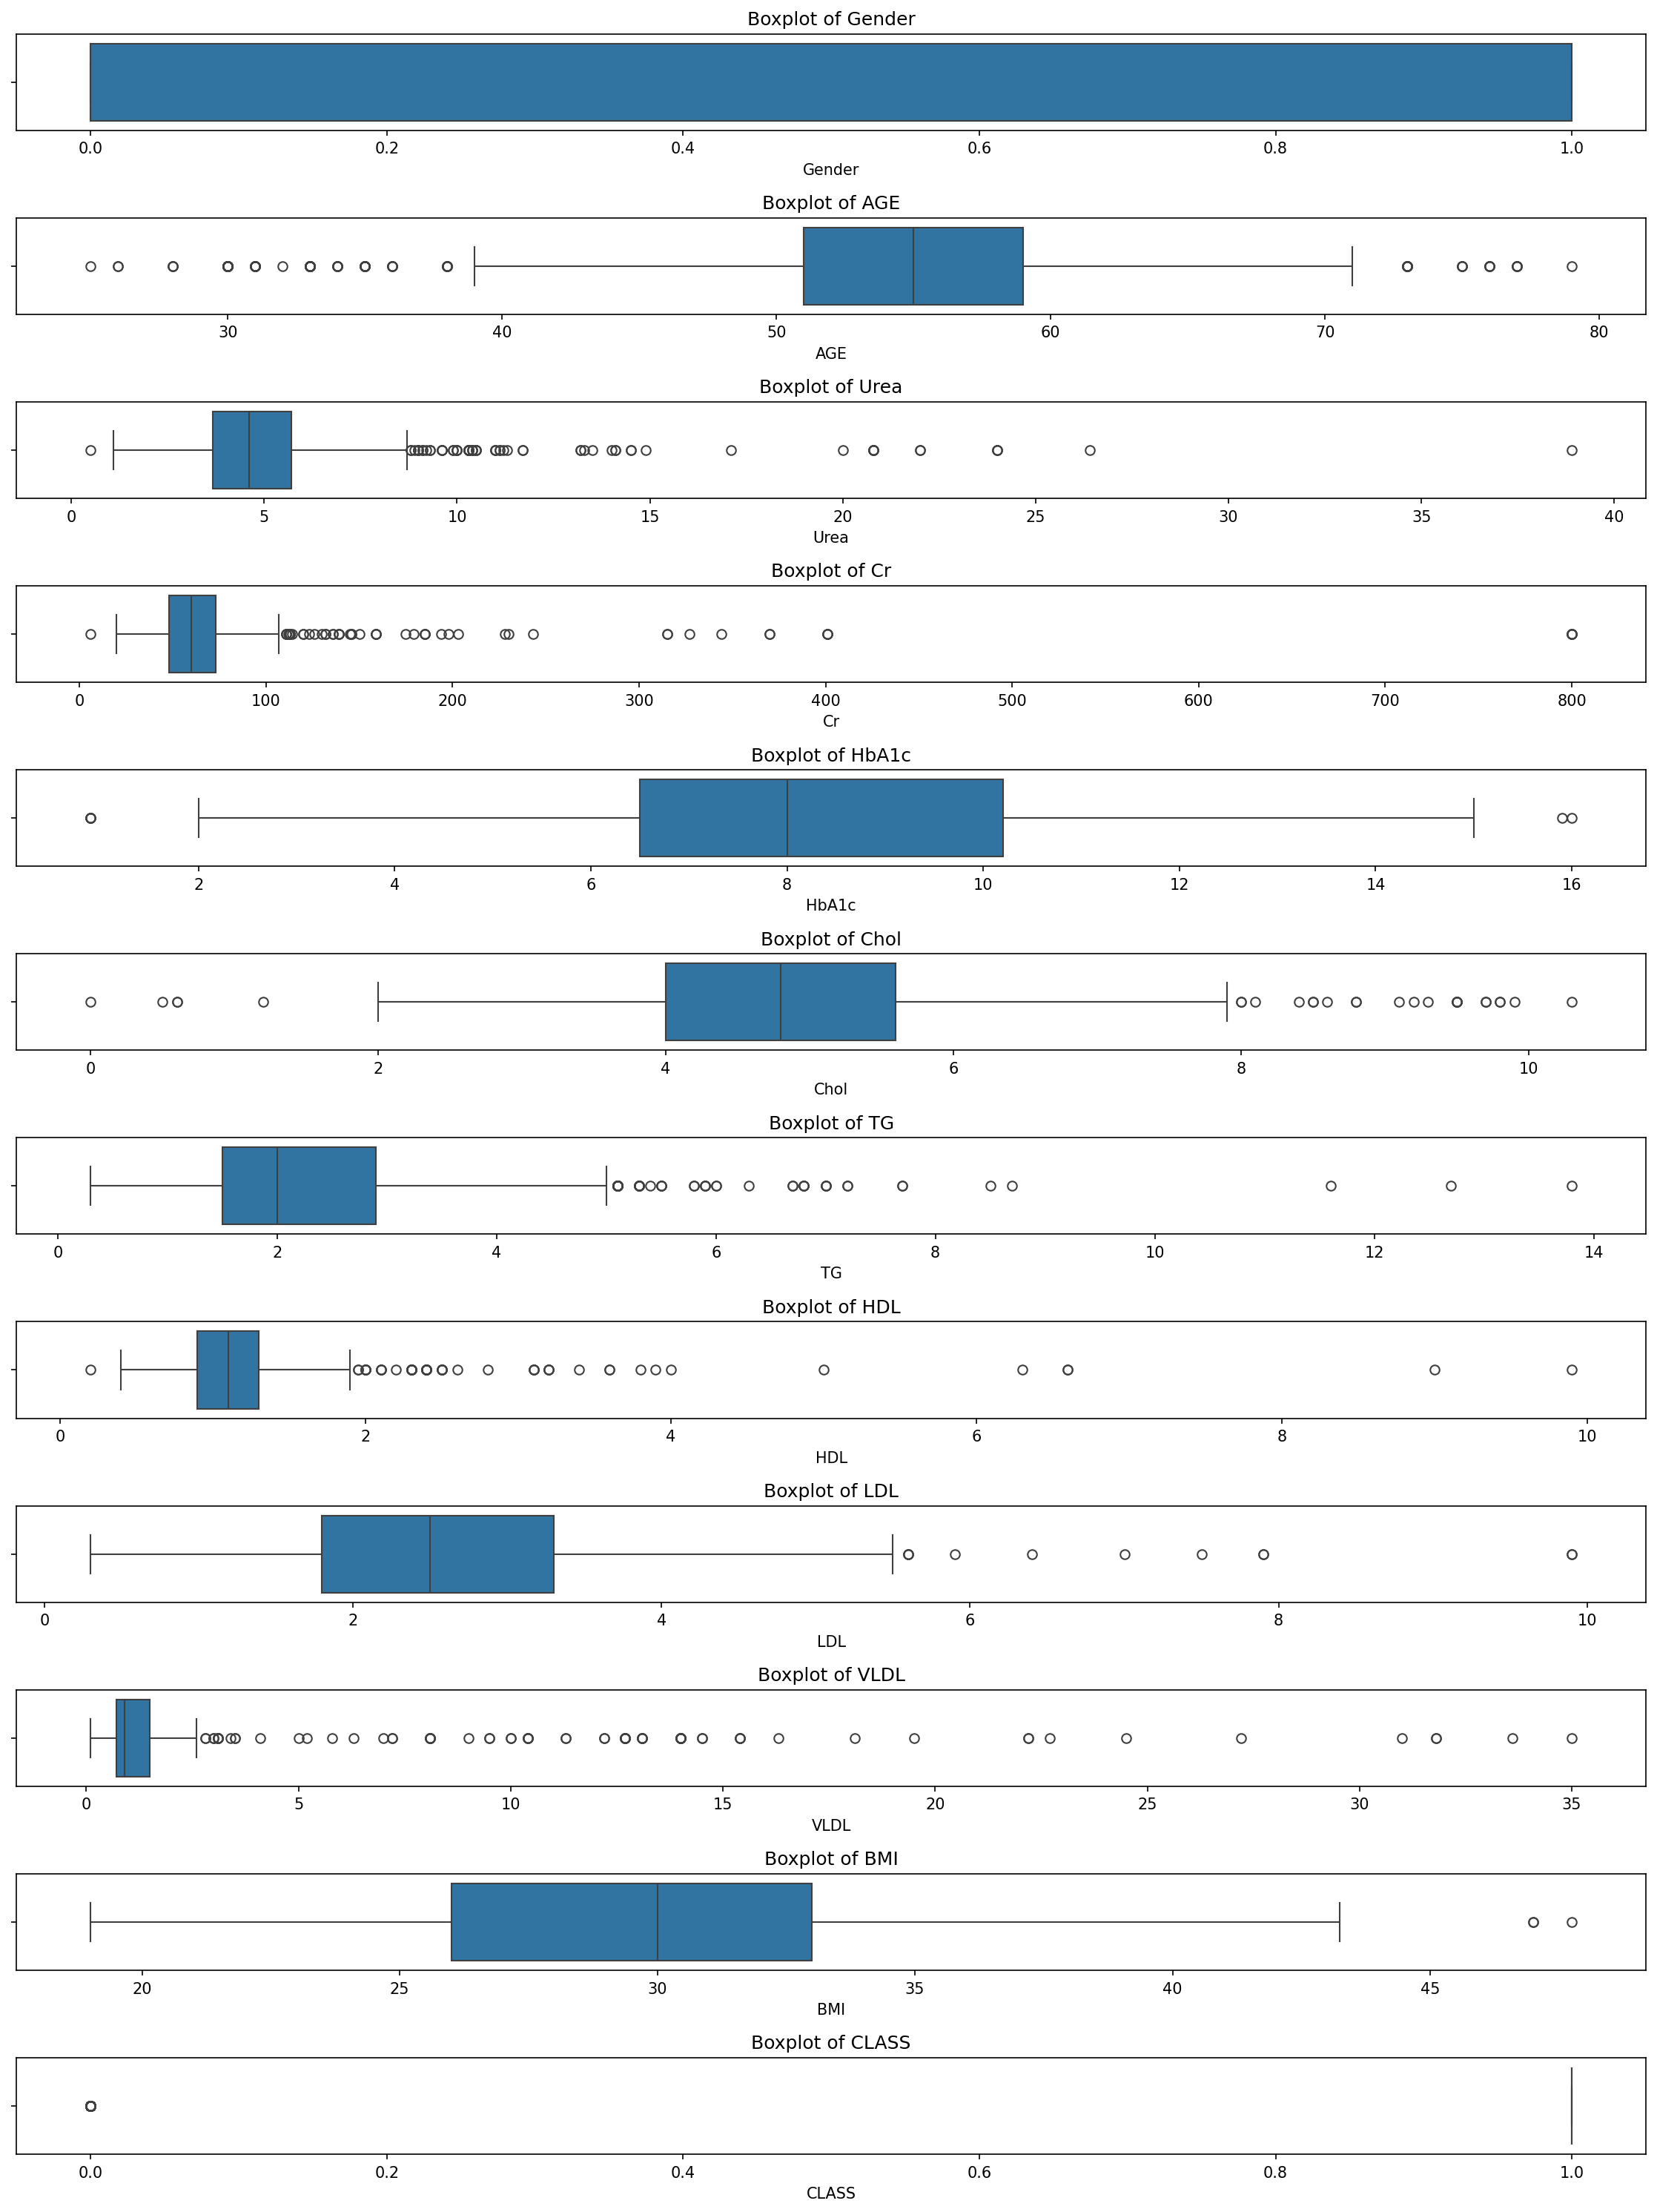
\includegraphics[width=\textwidth]{02_all_features_boxplots.png}
    \caption{Boxplots of all features in the cleaned dataset.}
    \label{fig:all_boxplots}
\end{figure}

\subsection{Correlation Analysis}

The correlation heatmap (Figure~\ref{fig:heatmap}) highlights the linear
associations between features. The strongest correlations with the target
variable CLASS are:

\begin{itemize}
    \item \textbf{HbA1c} --- the most predictive feature, directly measuring
          average blood glucose levels.
    \item \textbf{BMI} --- a strong secondary predictor; higher BMI is a known
          risk factor for type 2 diabetes.
    \item \textbf{AGE} --- older patients show a higher prevalence of diabetes
          in this dataset.
\end{itemize}

\begin{figure}[H]
    \centering
    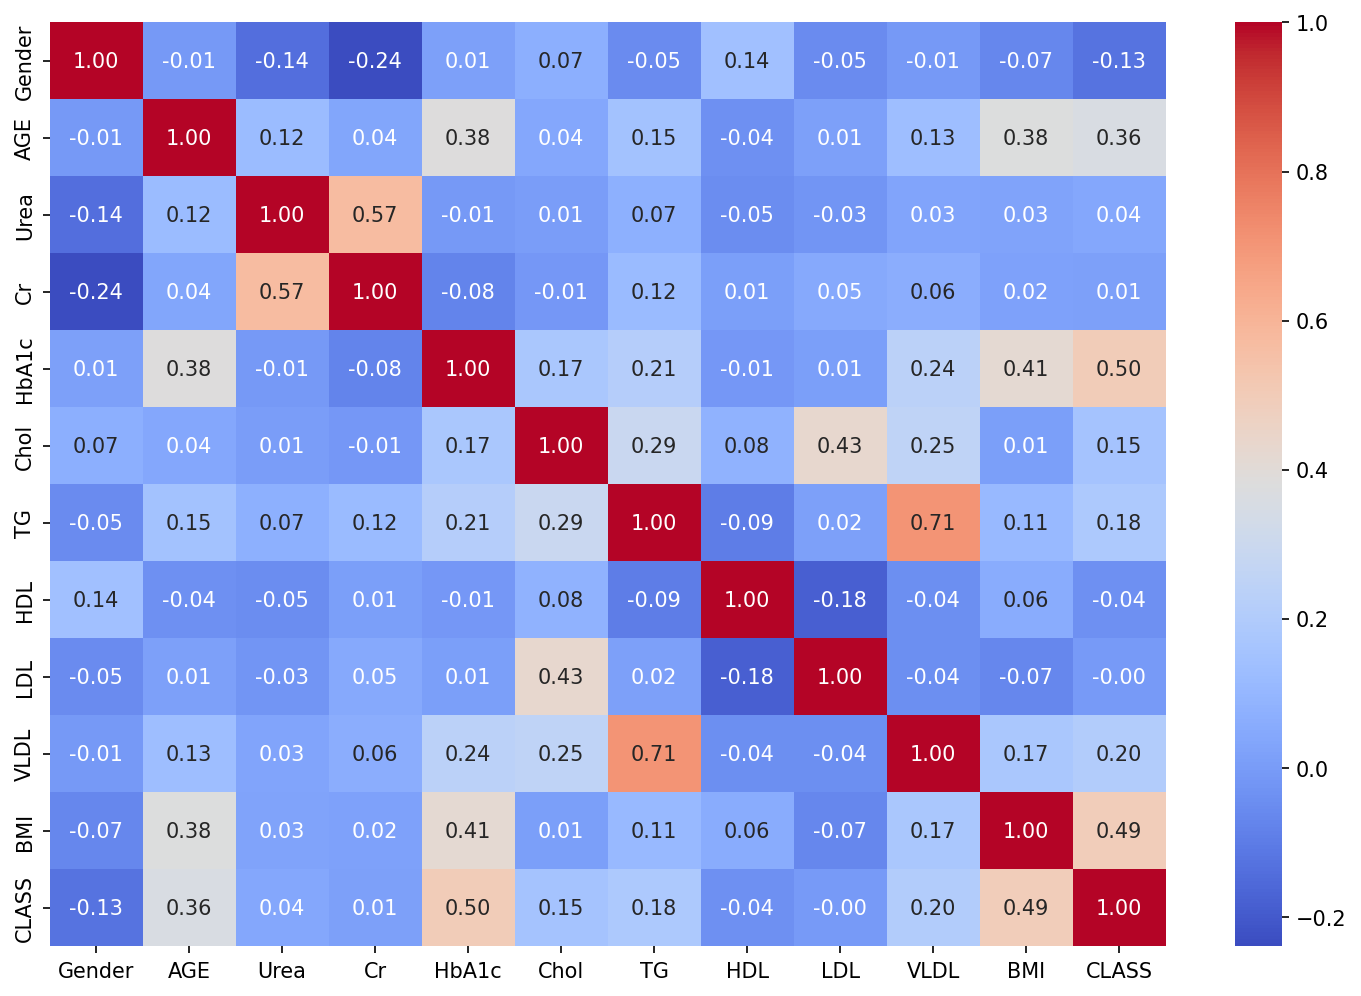
\includegraphics[width=\textwidth]{08_correlation_heatmap.png}
    \caption{Pearson correlation heatmap of all numeric features.}
    \label{fig:heatmap}
\end{figure}

% ══════════════════════════════════════════════════════════════════════════════
\section{Predictive Modelling}

\subsection{Train/Test Split}

The dataset was split into a training set (80\%, $n=779$) and a held-out test
set (20\%, $n=195$) using stratified sampling to preserve the class ratio.

\subsection{Class Balancing via Undersampling}
\label{sec:balancing}

Training directly on the imbalanced set risks producing models biased towards
predicting the majority class (diabetic). To mitigate this, \textbf{random
undersampling} of the majority class was applied to the training set: 82
samples were drawn at random from the 697 diabetic training records to match
the 82 non-diabetic records, yielding a balanced training set of 164 samples
with a 50/50 split.

\subsection{Models}

Four classification algorithms were evaluated:

\begin{itemize}
    \item \textbf{Logistic Regression} --- linear probabilistic classifier.
    \item \textbf{Decision Tree} --- non-linear, tree-based, highly 
          interpretable.
    \item \textbf{K-Nearest Neighbours (KNN)} --- instance-based, captures
          local patterns.
    \item \textbf{Random Forest} --- ensemble of decision trees; robust and
          typically high-performing.
\end{itemize}

Each model was trained and evaluated under both the imbalanced and balanced
training conditions, always tested on the same held-out test set.

\subsection{Results}

Tables~\ref{tab:metrics_bal} and~\ref{tab:metrics_imb} report the performance
metrics on the test set. Figure~\ref{fig:metrics_bar} shows the metrics
comparison for the balanced training set visually, while
Figure~\ref{fig:pointplots} tracks how each metric changes from imbalanced to
balanced training.

\begin{table}[H]
\centering
\caption{Test-set performance metrics --- \textbf{balanced} training set.}
\label{tab:metrics_bal}
\renewcommand{\arraystretch}{1.3}
\begin{tabular}{lccccc}
\toprule
\textbf{Model} & \textbf{Accuracy} & \textbf{Precision} & \textbf{F1-Score}
               & \textbf{Recall (0)} & \textbf{Recall (1)} \\
\midrule
Logistic Regression & 0.959 & 0.994 & 0.977 & 0.950 & 0.960 \\
Decision Tree       & \textbf{0.995} & \textbf{1.000} & \textbf{0.997} & \textbf{1.000} & 0.994 \\
KNN                 & 0.872 & 0.975 & 0.925 & 0.800 & 0.880 \\
Random Forest       & 0.985 & \textbf{1.000} & 0.991 & \textbf{1.000} & 0.983 \\
\bottomrule
\end{tabular}
\end{table}

\begin{table}[H]
\centering
\caption{Test-set performance metrics --- \textbf{imbalanced} training set.}
\label{tab:metrics_imb}
\renewcommand{\arraystretch}{1.3}
\begin{tabular}{lccccc}
\toprule
\textbf{Model} & \textbf{Accuracy} & \textbf{Precision} & \textbf{F1-Score}
               & \textbf{Recall (0)} & \textbf{Recall (1)} \\
\midrule
Logistic Regression & 0.959 & 0.972 & 0.977 & 0.750 & 0.983 \\
Decision Tree       & \textbf{0.995} & 0.994 & \textbf{0.997} & 0.950 & \textbf{1.000} \\
KNN                 & 0.923 & 0.935 & 0.958 & 0.400 & 0.983 \\
Random Forest       & \textbf{0.995} & 0.994 & \textbf{0.997} & 0.950 & \textbf{1.000} \\
\bottomrule
\end{tabular}
\end{table}

\begin{figure}[H]
    \centering
    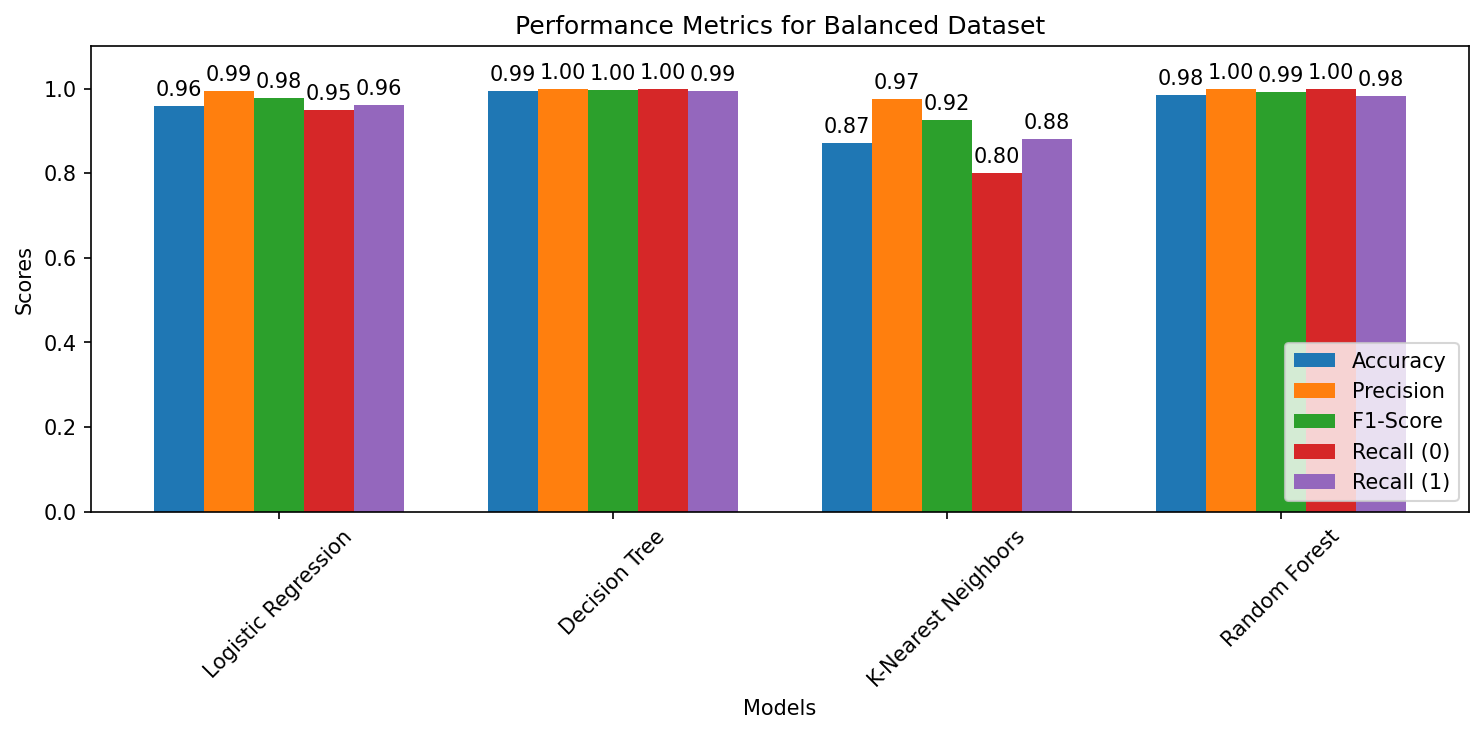
\includegraphics[width=\textwidth]{02_metrics_bar_balanced.png}
    \caption{Grouped bar chart of all metrics for each model trained on the
             balanced dataset.}
    \label{fig:metrics_bar}
\end{figure}

\begin{figure}[H]
    \centering
    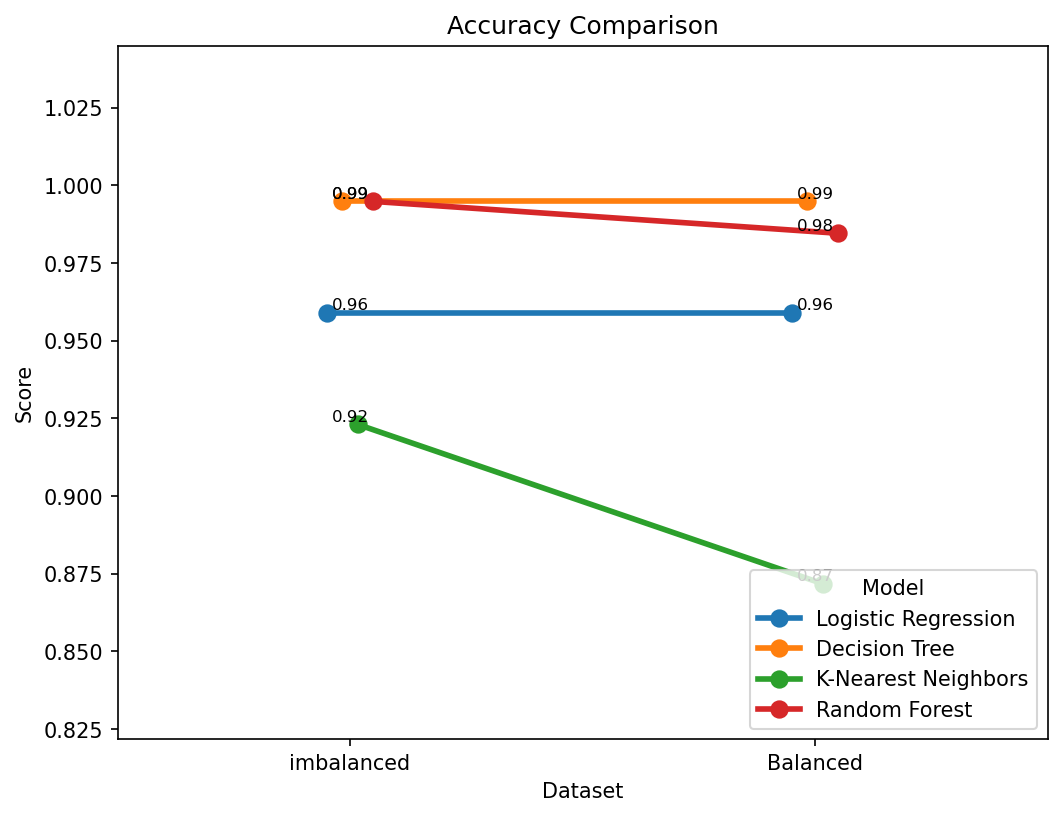
\includegraphics[width=\textwidth]{../pred/01_pointplot_Accuracy.png}
    \caption{Accuracy comparison across models: imbalanced vs.\ balanced
             training.}
    \label{fig:pointplots}
\end{figure}

\subsection{Confusion Matrices}

Figures~\ref{fig:cm_bal} and~\ref{fig:cm_imb} display the confusion matrices
for all four models under both training conditions.

\begin{figure}[H]
    \centering
    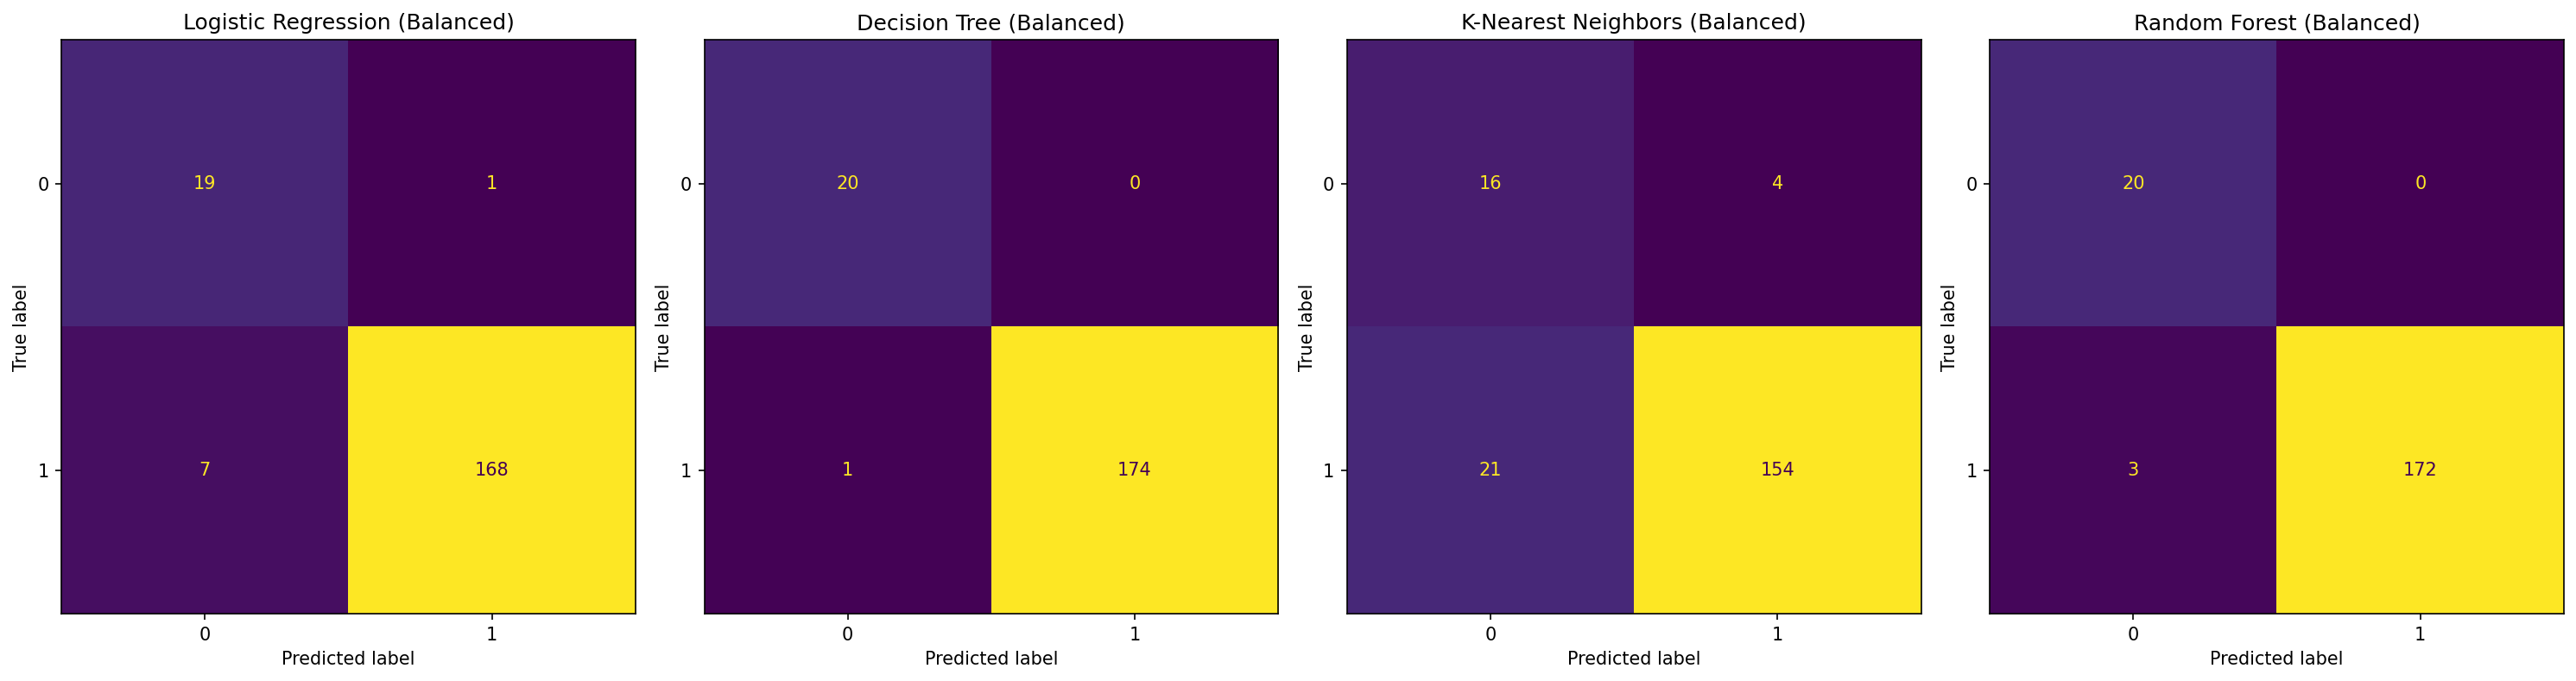
\includegraphics[width=\textwidth]{05_confusion_matrices_balanced.png}
    \caption{Confusion matrices --- models trained on the \textbf{balanced}
             training set.}
    \label{fig:cm_bal}
\end{figure}

\begin{figure}[H]
    \centering
    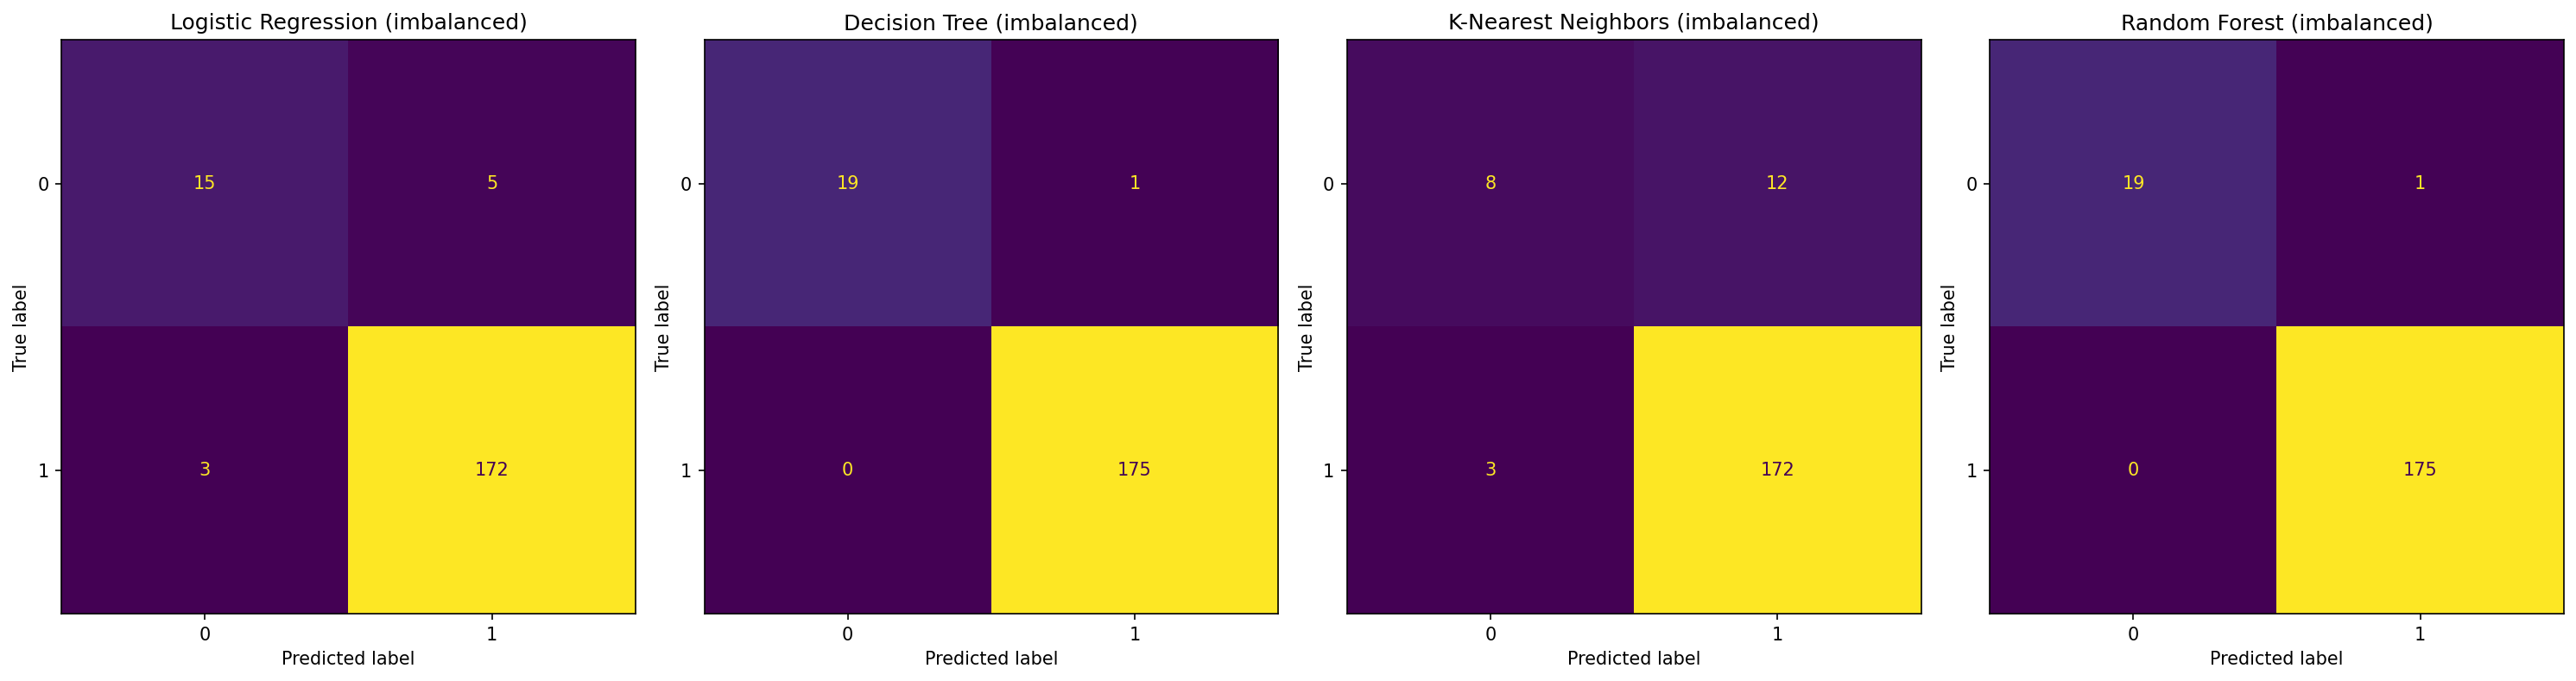
\includegraphics[width=\textwidth]{04_confusion_matrices_imbalanced.png}
    \caption{Confusion matrices --- models trained on the \textbf{imbalanced}
             training set.}
    \label{fig:cm_imb}
\end{figure}

\subsection{Feature Importance}

Figure~\ref{fig:feat_imp} shows the feature importances extracted from the
Random Forest model trained on the balanced dataset. \textbf{HbA1c} is by far
the most discriminative feature, confirming the EDA findings. BMI and AGE rank
second and third, consistent with the correlation analysis.

\begin{figure}[H]
    \centering
    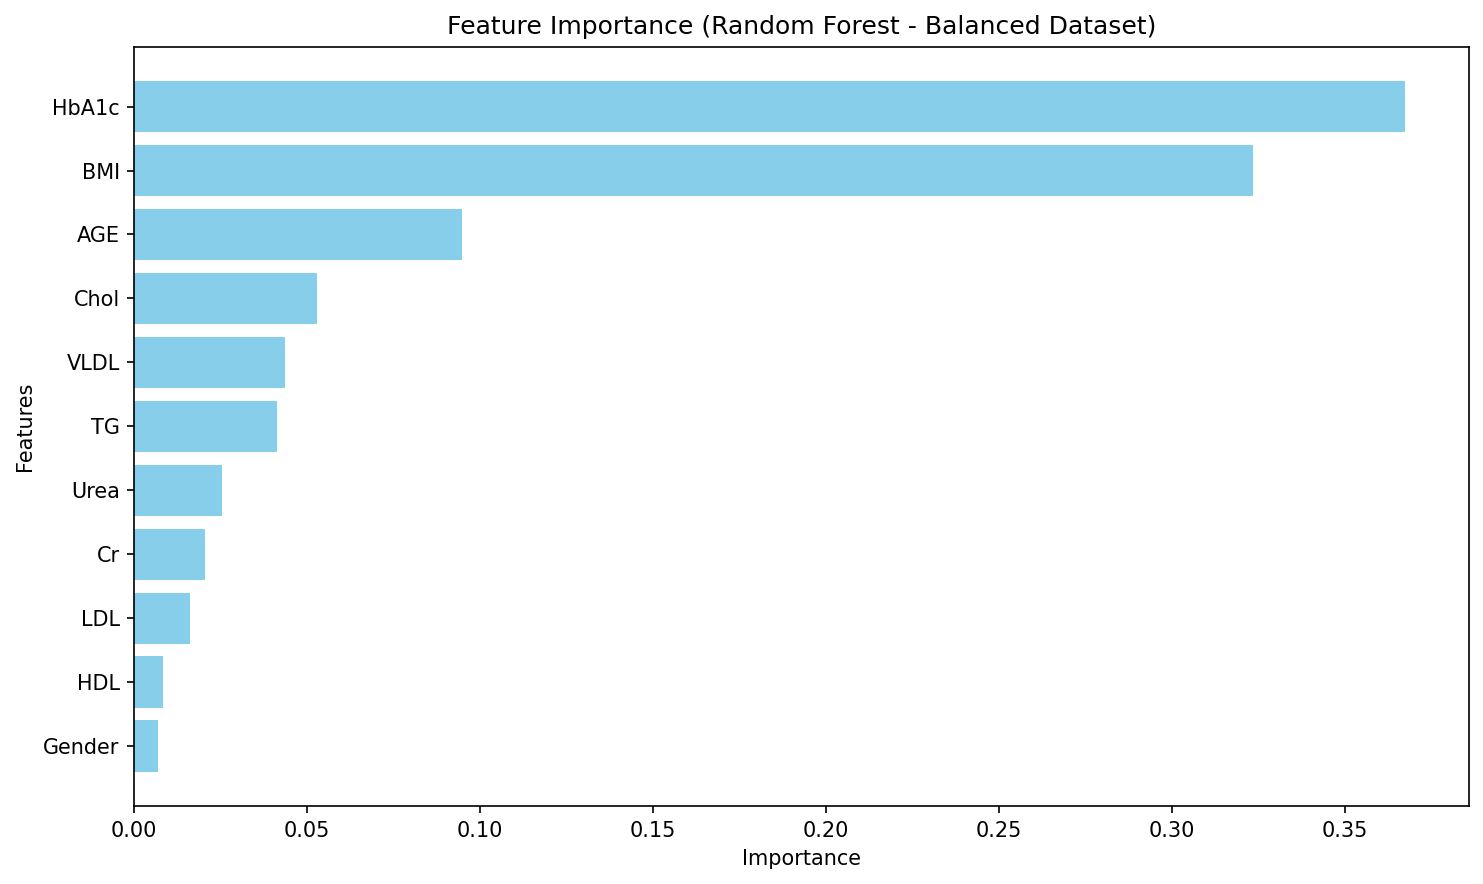
\includegraphics[width=0.8\textwidth]{03_feature_importance.png}
    \caption{Feature importances from the Random Forest classifier (balanced
             training set).}
    \label{fig:feat_imp}
\end{figure}

\subsection{Discussion}

The key observations from the modelling phase are:

\begin{itemize}
    \item \textbf{Decision Tree} and \textbf{Random Forest} achieve near-perfect
          performance ($\text{accuracy} = 99.5\%$, $F_1 \approx 0.997$) on this
          dataset under both training conditions. The high scores are partly
          attributable to the strong separability provided by HbA1c.
    \item \textbf{Balancing improves minority-class recall}: the most visible
          impact of undersampling is on \textit{Recall (0)} --- i.e., the
          ability to correctly identify non-diabetic patients. Logistic
          Regression's Recall (0) improves from 0.750 (imbalanced) to 0.950
          (balanced), and KNN's from 0.400 to 0.800. This is clinically
          significant: failing to identify a true non-diabetic is a
          false positive that carries real consequences.
    \item \textbf{KNN} is the weakest performer across all conditions, likely
          because it is sensitive to the feature scale and the high class
          imbalance in the original data.
\end{itemize}

% ══════════════════════════════════════════════════════════════════════════════
\section{Streamlit Web Application}

An interactive web application built with
\href{https://streamlit.io}{Streamlit} was developed to make the full pipeline
accessible without requiring any programming knowledge. The app is located in
\texttt{src/ST\_EDA\_prediction.py} and can be launched with:

\begin{lstlisting}
cd src
streamlit run ST_EDA_prediction.py
\end{lstlisting}

The application is divided into the following sections:

\begin{itemize}
    \item \textbf{Dataset Overview} --- raw data preview and summary statistics.
    \item \textbf{Data Cleaning} --- step-by-step walkthrough of the cleaning
          pipeline, with live tables and charts for each step.
    \item \textbf{Outlier Detection} --- interactive boxplots with physiological
          threshold lines.
    \item \textbf{VLDL/TG Analysis} --- scatter plots illustrating the
          unit-inconsistency discovery and correction.
    \item \textbf{EDA} --- gender distribution, class distribution, age KDE,
          interactive feature selector, scatterplot builder, correlation
          heatmap, and key-feature boxplots by class.
    \item \textbf{Model Training \& Benchmarking} --- trains all four models,
          displays metric tables and pointplots for both balanced and imbalanced
          conditions.
    \item \textbf{Prediction} --- a form for entering patient data (age, gender,
          blood markers, BMI) and receiving real-time predictions from all four
          models simultaneously.
\end{itemize}

% ══════════════════════════════════════════════════════════════════════════════
\section{Conclusions}

This project demonstrated a complete end-to-end data science workflow on a
real healthcare dataset:

\begin{enumerate}
    \item A thorough cleaning pipeline resolved missing values, encoding
          inconsistencies, physiologically implausible outliers, and a
          unit-measurement error in the VLDL column.
    \item EDA confirmed that \textbf{HbA1c}, \textbf{BMI}, and \textbf{AGE} are
          the most informative predictors of diabetes in this dataset.
    \item Among the four classifiers evaluated, \textbf{Decision Tree} and
          \textbf{Random Forest} achieved the best overall performance
          ($F_1 \approx 0.997$). Balancing the training set is crucial for
          improving recall on the minority (non-diabetic) class —- particularly
          relevant in a medical screening context.
    \item The Streamlit application provides an intuitive interface for
          non-technical users to explore the data and obtain real-time
          predictions.
\end{enumerate}

\vspace{1em}
\noindent\textit{Disclaimer: this project is a technical demonstration of an
ML workflow on healthcare-style data. Results must not be used for medical
diagnosis or treatment.}

\end{document}
